\subsection{Konfiguration mit STM32CubeMX}
\label{sec:CubeMX}

In den nachfolgenden Unterkapiteln sind die Konfigurationen in der STM32CubeMX Software abgebildet und beschrieben. Zudem sind Code Beispiele aufgeführt, die zeigen, wie die konfigurierte Peripherie im Projekt verwendet wird.

In der Abbildung \ref{pic:CubeMX_Pinout} ist das Pinout des STM32F412 ersichtlich.


\begin{figure}[H]
	\centering
	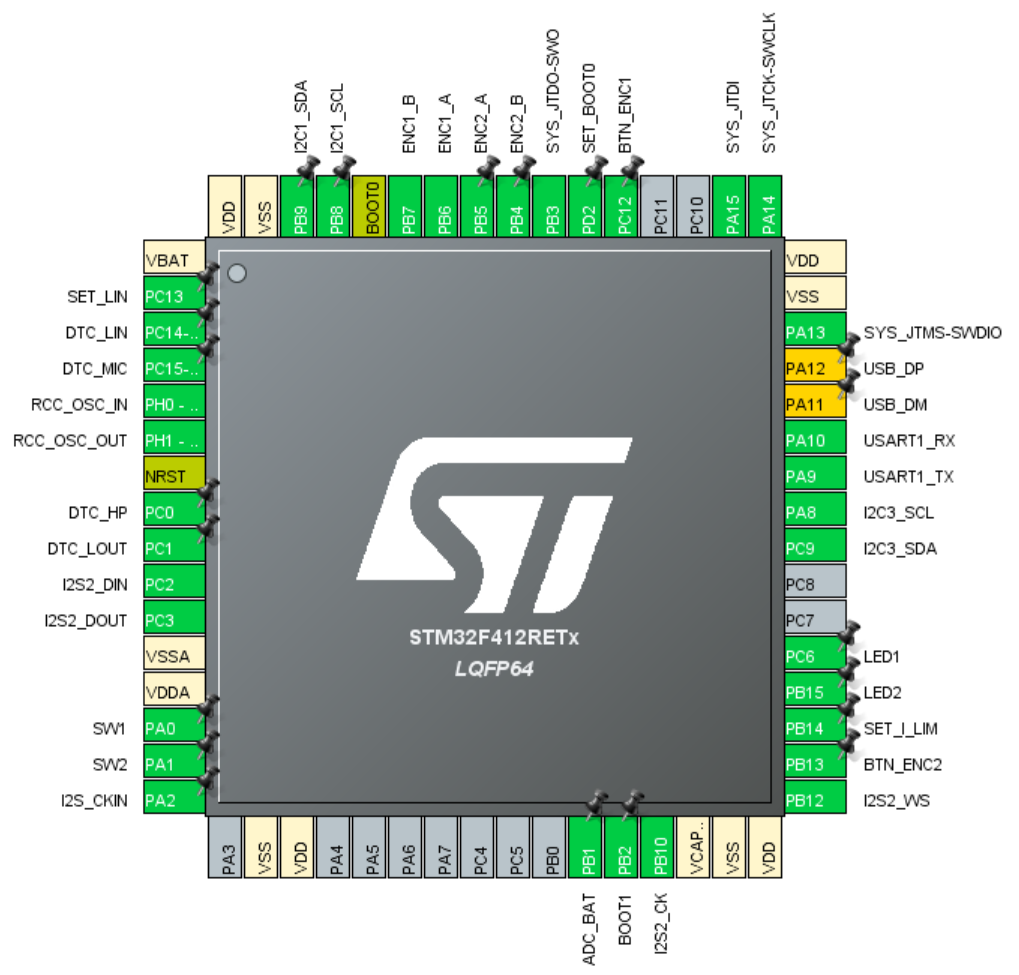
\includegraphics[width=0.9\linewidth]{CubeMX_Pinout}
	\caption{Pinout des STM32F412 in STM32CubeMX}
	\label{pic:CubeMX_Pinout}
\end{figure}




